\begin{savequote}[75mm] 
By failing to prepare, you are preparing to fail.
\qauthor{Benjamin Franklin} 
\end{savequote}

\chapter{Summarization approaches}
\label{chap:app}


%TODO introduction 

In this chapter, we will discuss different approaches of \ac{ats}. 
According to \citet{12-nenkova-mckeown}, topic representation approach contains topic words, frequency driven, latent semantic analysis, etc. 
We are, rather, interested in the nature of used resources.
Are they dependent on a specific language? or domain? do the methods need a lot of resources?
This is why we follow their other taxonomy \citep{11-nenkova-mckeown} called ``Semantics and discourse" which we present as ``linguistic approach" since its methods as highly connected to the language being processed.
The taxonomy of \citet{12-lloret-palomar} seems to approach our vision. 
The difference is that we consider topic-based and discourse-based approaches as sub-approaches of linguistic one, since the two are based on linguistic properties of the input text.

\section{Statistical approach}

Statistical approach has been used in ATS since its first days. 
It is based on some features which are used to score the relevancy of text units (generally, sentences) to the main topic or users requests. 
%These features can be combined to score the units using many aspects, and get the highest scored ones.
Usually, to score a unit many statistical features are used as shown in equation \ref{eq:combin-crit}.
\begin{equation}
	\label{eq:combin-crit}
	Score(s_i) = \sum_{f \in F}{\alpha_f * Score_f(s_i)}
\end{equation}
Where $ \alpha_f $ is the weight of a feature $ f $ in the features set $ F $.
The features weights can be fixed manually or using machine learning techniques.
Also, other methods such as optimization can be used. 
For instance, \citep{17-feigenblat-al} propose an unsupervised query-focused multi-document summarization method based on Cross-Entropy (CE) method \citep{04-rubinstein-kroese}. 
It seeks to select a subset of sentences that maximizes a given quality target function using some statistical features.


\subsection{Term frequency (TF)}

\ac{tf} is the oldest feature \citep{58-luhn} and the most famous one. 
In his work, the terms frequency used to measure significant words, which has to be between two thresholds to ensure that the term is important yet not specific to the text's domain.
It supposes that frequently repeated terms in a text are important.
This feature is still being used in conjunction of machine learning, such as the work of \citet{17-yousefiAzar-hamey}.

\ac{tf} has a problem when it comes to domain-relative words; For example, in documents talking about computer science, certain words such as ``computer" will have great frequencies even if they do not represent the main topic.
To address this problem, \citet{58-luhn} uses two thresholds to ensure that the term is important yet not specific to the document's domain.
A more advanced solution is to use \ac{tfidf} which is first defined by \citet{73-salton-yang}.
Given a corpus $ D $ containing many documents $ d \in D $, the measure \ac{idf} is calculated as shown in Equation~\ref{eq:idf}.
\begin{equation}
	\label{eq:idf}
	idf(t) = log{\frac{|D|}{|\{d \in D /\ t \in d\}|+1}}
\end{equation}
Where: 
$ |D| $ is the number of documents in corpus $ D $;
$ |\{d \in D /\ t \in d\}| $ is the number of documents containing the term $ t $.

\subsection{Position in the text}

The position of words \citep{58-luhn} and sentences \citep{58-baxendale,69-edmundson} in a text has good potential of capturing their importance. 
In \citep{58-luhn}, the position of words in a sentence is used to create some sort of groups, where each one is the set of significant words separated by at most 5 to 6 non-significant words. 
Then, the group which has the most significant words is used to score the sentence, as shown in Figure \ref{fig:luhn-score}.

\begin{figure}[!ht]
	\centering
	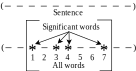
\includegraphics[width=50mm]{figures/approaches/luhn-score.pdf} % % %[width=140mm]
	\caption{Luhn score using word position \citep{58-luhn}.}
	\label{fig:luhn-score}
\end{figure}

The position of sentences in a text is used as indicator of its importance: the first and the last sentences tend to be more informative than the others \citep{69-edmundson}.
For instance, in scientific articles, sentences from the  introduction and the conclusion contain more information about the topic than other sentences.
In \citep{58-baxendale}, it is established that the first and the last sentences in paragraphs are more important. 
The author used a corpus of 200 paragraphs to test the importance of sentences according to their positions in a paragraph. 
He found out that in 85\% of these paragraphs, the first sentence is the most important; and that in 7\% of them the last one is.
Afterward, \citet{69-edmundson} formulated a hypothesis that sentences which appear very soon or late in the document or paragraphs have a good chance to be topic sentences.

Position feature can be used differently to score sentences.
\citet{04-nobata-sekine} define three methods to score a sentence $ s_i $, where $ i $ is its position in a document of $ n $ sentences.
The first method Equation (\ref{eq:nobota-pos-1}) supposes that only the first sentences less than a defined position $ N $ are important.
\begin{equation}
\label{eq:nobota-pos-1}
Score_{pos}(s_i) = \left\lbrace 
\begin{array}{lll}
1 & if & (i < N) \\
0 & otherwise & \\
\end{array}
\right. 
\end{equation}
The second method (Equation \ref{eq:nobota-pos-2}) supposes that a sentence's importance is inversely proportional to its position.
\begin{equation}
\label{eq:nobota-pos-2}
Score_{pos}(s_i) = \frac{1}{i}
\end{equation}
The last method (Equation \ref{eq:nobota-pos-3}) supposes that the first and the last sentences are more important.
\begin{equation}
\label{eq:nobota-pos-3}
Score_{pos}(s_i) = \max(\frac{1}{i}, \frac{1}{n-i+1})
\end{equation}
According to the authors, the second method gives the best results among the three.
%
\citet{09-abdelfattah-ren} use the position of sentences in paragraphs instead of the whole text. 
They suppose that the 5 first sentences in a paragraph are the most important (Equation \ref{eq:abdelfattah-pos}).
\begin{equation}
\label{eq:abdelfattah-pos}
Score_{pos}(s_i) = \left\lbrace 
\begin{array}{lll}
6 - i & if & (i \leq 5)\\
0 & otherwise &  \\
\end{array}
\right. 
\end{equation}
Where: $ i $ is the position of the sentence in the paragraph.

Like Luhn, \citet{10-ouyang-al} use word position based on the hypothesis that a word is more informative if it appears earlier in the text.
Therefore, the position of a word can be calculated according to its other occurrences in the whole text and not just according to other words in the sentence.
For that, four different functions are defined: Direct proportion (DP), Inverse proportion (IP), Geometric sequence (GS) and Binary function (BF). 
Direct proportion (DP) attributes a score of $ 1 $ of the first appearance and $ 1/n $ to the last one as, where $ n $ is the count of words in the sentence. 
Then the function to calculate DP is given in Equation \ref{eq:p_dp}, where $ i $ is the position of the word in the sentence. 
\begin{equation}
\label{eq:p_dp}
f_{DB}(i) = \frac{(n - i +1)}{n}
\end{equation}
Inverse proportion (IP) function is given in Equation \ref{eq:p_ip}, where the degree decreases quickly at smaller positions. This gives advantage to leading sentences. 
\begin{equation}
\label{eq:p_ip}
f_{DB}(i) = \frac{1}{i}
\end{equation}
Geometric sequence (GS) function scores an appearance of a word as the sum of the scores of all its following appearances (Equation \ref{eq:p_gs}).
\begin{equation}
\label{eq:p_gs}
f_{GS} (i) = (1/2)^{i-1}
\end{equation}
Binary function (BF) affords more importance to the first appearance of a word, and the others an equally less importance.
Therefore the first one will get a score of $ 1 $ and the others a score of a given $ \lambda \ll 1 $ as shown in Equation \ref{eq:p_bf}.
\begin{equation}
\label{eq:p_bf}
f_{BF} (i) = \left\lbrace 
\begin{array}{lll}
1 & if & i = 1\\
\lambda & otherwise &  \\
\end{array}
\right. 
\end{equation}
The final score is calculated as shown in Equation \ref{eq:ouyang-pos} 
\begin{equation}
\label{eq:ouyang-pos}
Score(s) = \sum\limits_{w_i \in s} \frac{\log(freq(w_i)) * pos(w_i)}{|s|} 
\end{equation}
Where $ pos(w_i) $ is one of the four functions shown previously; $ freq(w_i) $ is the frequency of the word $ w_i $; $ |s| $ is the length of the sentence.

\subsection{Title and subtitle words}

``The title carries the topic of the document", this hypothesis was first introduced by \citet{69-edmundson}.
When we divide a document into sections and subsections, we choose representative titles for each. 
So, any sentence containing some words of a title is considered as important.
This feature can be treated as if the title was a request \citep{88-salton-buckley}. 

\citet{01-ishikawa-al} fuse this feature with term frequency, in a way that the frequencies of the title words are weighted more than regular words.
In Equation \ref{eq:ishikawa-head}, a sentence $ s_i $ is scored by the frequencies of its words $ w $; if the word belongs to the title, its frequency is multiplied by a number $ A > 1 $ (the authors used $ A = 3 $).
%\begin{equation}
%\label{eq:ishikawa-head}
%Score_{title}(s_i) = \sum_{\{w\} \in s_i}{\alpha(w) * tf(w)}
%\end{equation}
%Where: 
%\[ 
%\alpha(w) = \left\lbrace 
%\begin{array}{lll}
%A > 1 & if & w \in title \\
%1 & otherwise & \\
%\end{array} 
%\right. 
%\]
\begin{equation}
	\label{eq:ishikawa-head}
	Score_{title}(s_i) = \sum_{\{w\} \in s_i}{\alpha(w) * tf(w)} 
	\text{ where }
	\alpha(w) = \left\lbrace 
	\begin{array}{ll}
		A > 1 & \text{if } w \in title \\
		1 & otherwise \\
	\end{array} 
	\right. 
\end{equation}
%%04-nobata-sekine
To score sentences based on title's words, \citet{04-nobata-sekine} propose two methods.
The first method uses $ tf*idf $ of the title's words $ T $ as indicated in Equation \ref{eq:nobta-head-1}.
\begin{equation}
\label{eq:nobta-head-1}
Score_{title}(s_i) = \frac{\sum_{w \in T \bigcap s_i}{\frac{tf(w)}{tf(w)+1} idf(w)}}
{\sum_{w \in T}{\frac{tf(w)}{tf(w)+1} idf(w)}}
\end{equation}
The second method uses named entities $ e $ and frequencies of words $ tf $ as shows in Equation \ref{eq:nobta-head-2}.
\begin{equation}
\label{eq:nobta-head-2}
Score_{title}(s_i) = \frac{\sum_{e \in T \bigcap s_i}{\frac{tf(e)}{tf(e)+1}}}
{\sum_{e \in T}{\frac{tf(e)}{tf(e)+1}}}
\end{equation}
According to the authors, the second method gives better results.

\subsection{Sentence length}

This feature was used to penalize too short sentences \citep{95-kupiec-al}.
Given a threshold, for example 5 words, the feature is true if it exceeds this threshold and false otherwise.
Sentences which are very small, in number of words, are unlikely to be important so it is better to omit them.
A more complex formula to score a sentence is expressed in the two methods proposed by \citet{04-nobata-sekine}.
The first method scores a sentence based on its length and a predefined maximum value $ L_{max} $ as shown in Equation \ref{eq:nobota-len-1}.
\begin{equation}
\label{eq:nobota-len-1}
Score_{length}(s_i) = \left\lbrace 
\begin{array}{lll}
\frac{|s_i|}{L_{max}} & if & (|s_i| \leq L_{max}) \\
1 & otherwise & \\
\end{array}
\right. 
\end{equation}
The second, which gives better results, affords a negative score to penalize sentences shorter than a predefined minimum value $ L_{min}$ (Equation \ref{eq:nobota-len-2}).
\begin{equation}
\label{eq:nobota-len-2}
Score_{length}(s_i) = \left\lbrace 
\begin{array}{lll}
0 & if & (|s_i| \geq L_{min}) \\
\frac{|s_i| - L_{min}}{L_{min}} & otherwise & \\
\end{array}
\right. 
\end{equation}
As observed by the authors, the second method is the best.

A more recent formula proposed by \citet{09-abdelfattah-ren} is indicated in Equation \ref{eq:abdelfattah-len}.
It scores a sentence $ s_i $ using its words number $ |s_i| $, the document's words number $ |d| $ and the number of sentences in this document $ |\{s: s \in d\}| $.
\begin{equation}
	\label{eq:abdelfattah-len}
	Score_{length}(s_i) = \frac{|s_i| * |\{s: s \in d\}|}{|d|}
\end{equation} 


\subsection{Centroid}

A centroid, as defined by \citet{04-radev-al}, is ``\textit{a set of words that are statistically important to a cluster of documents}". 
Since it is the most important in the cluster, the documents and sentences containing it are also important.
One famous summarization system using clusters centroid to extract summaries is MEAD \citep{00-radev-al,04-radev-al}.
MEAD is a multi-document summarizer, where similar documents to the centroid are clustered together.
Then, a set of parameters (Centroid value, Positional value, and First-sentence overlap) are used to rank each sentence from the resulting cluster.
The centroid value $ C_i $ for a sentence $ S_i $ is computed as in Equation \ref{eq:centroid}.
\begin{equation}
\label{eq:centroid}
C_i = \sum_{w \in S_i}  C_{w,i}
\end{equation}
Where, $ C_{w,i} $ is the centroid value of a word $ w $ in sentence $ S_i $.
The positional value $ P_i $ for a sentence $ S_i $ is computed according to its position in the document with $ n $ sentences as in Equation~\ref{eq:centroid-p}.
\begin{equation}
\label{eq:centroid-p}
P_i = \frac{n - i + 1}{n} * C_{max}
\end{equation}
Where $ C_{max} $ is the maximum centroid score in that document.
The First-sentence overlap value $ F_i $ of a sentence $ S_i $ is given as in Equation~\ref{eq:centroid-f}.
\begin{equation}
\label{eq:centroid-f}
F_i = \overrightarrow{S_1} \overrightarrow{S_i}
\end{equation}
Where $ S_1 $ is the first sentence.
These three scores are combined into one score along with a redundancy score to extract the most scored sentences.

A more recent work presents an unsupervised centroid-based document-level reconstruction framework using distributed bag of words model \citep{18-mani-al}.
The method uses machine learning to construct a distributed bag of words (DBOW) model for each document. 
Then, the centroid $ C $ of a multi-document set $ D = [d_1, d_2, ..., d_n] $ is given in Equation~\ref{eq:centroid-mani}.
\begin{equation}
\label{eq:centroid-mani}
C = \frac{1}{|D|}\sum\limits_{1}^{|D|} DBOW(d_i)
\end{equation}
The summary is constructed by iteratively selecting the sentences with the minimum reconstruction error (error between summary's DBOW and $ C $).

\subsection{Frequent itemsets}

Frequent itemsets are common sets of items which have at least a minimum amount of times. 
It was, first, proposed by \citet{94-agrawal-srikant} to solve the problem of discovering association rules
between items in a large database of sales transactions.
In ATS, the itemsets are considered as sets of terms extracted from sentences, where those which co-occur in many sentences are considered as frequent itemsets.

\citet{12-baralis-al} apply an entropy-based strategy to generate compact itemset-based models, where each document sentence is seen as a separate transaction. 
They formalize the problem of selecting sentences as a set covering optimization problem.
It is solved by a greedy strategy where sentences covering the maximum number of itemsets are selected.
This method is ameliorated in MWI-Sum system \citep{15-baralis-al} by replacing traditional itemsets with weighted ones in order to increase item relevance in the mining process. 
Also, \ac{tfidf} is used as relevance score. 

This approach is used in \citep{17-litvak-vanetik} with the minimum description length (MDL) principle that employs
Krimp compression algorithm \citep{11-vreeken-al} for query-based \ac{ats}.
The key idea is to use the query to select related frequent itemsets (word sets).
It is, also, combined with other approaches such as: Latent Semantic Analysis \citep{19-cagliero-al}, graphs \citep{18-azadani-al}, clustering \citep{19-rouane-al}, etc.

\subsection{Latent semantic analysis (LSA)}

\ac{lsa} seeks to analyze relationships between a set of documents and the terms they contain.
It is used in \citep{04-steinberger-jezek} for text summarization. 
The algorithm starts by creating a matrix $ A $ of $ m $ rows representing the document terms, and $ n $ columns representing the sentences, where $ a_{i, j} \in A $ represents the frequency of the term $ i $ in the sentence $ j $. 
Then, the \ac{svd} of the matrix $ A $ is represented as in Equation \ref{eq:svd}.
\begin{equation}
	\label{eq:svd}
	A = U \varSigma V^T
\end{equation}
Where:
\begin{itemize}
	\item $ U = [u_{i,j}] $ is an $ m \times n $ column-orthonormal matrix whose columns are called left singular vectors.
	\item $ \varSigma = diag(\sigma 1, \sigma 2, ..., \sigma n) $ is an $ n \times n $ diagonal matrix, whose diagonal elements are non-negative singular values sorted in descending order
	\item $ V = [v_{i,j}] $ is an $ n \times n $ orthonormal matrix, whose columns are called right singular vectors.  
\end{itemize}
Then, the salience of a sentence $ k $ is given in equation \ref{eq:lsa}.
\begin{equation}
	\label{eq:lsa}
	s_k = \sqrt{\sum\limits_{i=1}^{n} v_{k,i}^2 . \sigma^2}
\end{equation}

%LSA recent works complete
\ac{lsa} can be used with other approaches such as frequent itemsets \citep{19-cagliero-al}. 
To overcome the inability of \ac{lsa} to consider the correlation between combinations of multiple-document
terms and the underlying concepts, the authors exploits frequent itemsets to describe all of the latent concepts covered by the documents.


%\subsection{Combination of features}
%
%Usually, to score a unit (sentence) not just one feature but many are used as shown in equation \ref{eq:combin-crit}.
%\begin{equation}
%	\label{eq:combin-crit}
%	Score(s_i) = \sum_{f \in F}{\alpha_f * Score_f(s_i)}
%\end{equation}
%Where $ \alpha_f $ is the weight of a feature $ f $ in the features set $ F $.
%%
%An early work which combine many features to score sentences is the work of \citet{69-edmundson}.
%The author used four features: Cue words (\textit{C: Cue}), term frequency (\textit{K: Key}), title words (\textit{T: Title}) and position (\textit{L: Location}).
%He used all the combinations of these features which gives 15 different combinations, where the weights are equal to 1.
%%Figure \ref{fig:edmundson-score} represents the mean co-selection scores (the percent of the number of pertinent sentences) of the most interesting combinations, and the interval between the min and the max.
%%\begin{figure}
%%\begin{center}
%%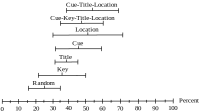
\includegraphics[width=.5\textwidth]{edmundson-score.pdf} % % %[width=140mm]
%% \caption{Mean co-selection scores of the features \citep{69-edmundson}.}
%% \label{fig:edmundson-score}
%%\end{center}
%%\end{figure}
%Most systems use different features combined together (linear combination, generally) to get a unique score. 
%The features weights can be fixed manually or using machine learning techniques described in a later section.
%%
%Also, other methods such as optimization can be used. 
%For instance, \citep{17-feigenblat-al} propose an unsupervised query-focused multi-document summarization method based on Cross-Entropy (CE) method \citep{04-rubinstein-kroese}. 
%It seeks to select a subset of sentences that maximizes a given quality target function using some statistical features.


\section{Graph-based approach}

%Introduce Graph-based approach
Inter-cohesion between text units (sentences) is an important property; A summary which contains linked units has the chance to be more pertinent to the input document's main topic.
Graph-based approach is based on transforming documents units (sentences, paragraphs, etc.) into a graph using a similarity measure, then this structure is used to calculate the importance of each unit. 
We divide graph-based works into two categories: those using graph properties such as the number of neighbors, and those iterating over the graph and changing nodes' scores till reaching a stable graph representation.

\subsection{Graph properties}

In \citep{97-salton-al}, document paragraphs are used to construct a graph of similarities, where each paragraph represents a node.
A paragraph is connected to another when their similarity is above a given threshold.
The authors define a feature called bushiness which is the number of a node's connections. 
The most scored paragraphs in term of bushiness are extracted to form a summary.

Node's bushiness can be used to score sentences alongside other statistical features \citep{09-abdelfattah-ren}.
In a graph of similarities between sentences, the importance of a sentence is the number of arcs connected to it.
Equation~\ref{eq:abdelfattah-arcs} represents the score based on number of arcs, where $ G =  \{S, A\} $ is the graph of similarities between the sentences, $ S $ is the set of sentences and $ A $ is the set of arcs.
\begin{equation}
	\label{eq:abdelfattah-arcs}
	Score_{\#arcs}(s_i) = |\{ s_j : a(s_i, s_j) \in A / s_j \in S, s_i \neq s_j \}|
\end{equation}

Beside bushy path of the node, \citet{14-ferreira-al} define another property called ``Aggregate Similarity". 
Instead of counting the number of arcs connected to a node, their weights are summed to represent this node's importance.
In their work, the authors investigate the fusion of multiple features, either graph-based or sentence features.

\subsection{Iterative graph}

LexRank \citep{04-erkan-radev} and TextRank \citep{04-mihalcea-tarau} are the most popular methods using graph-based summarization approach. 
The two methods use a modified version of PageRank \citep{98-brin-page} in order to score sentences. 
%
LexRank method \citep{04-erkan-radev} uses cosine similarity to construct a weighted graph where the nodes with a weight (similarity) less than a given threshold are omitted. 
Their method's continuous version follows almost the same equation as of TextRank, but it uses a \ac{tfidf} based cosine similarity instead.
%\begin{figure}[!ht]
%	\begin{center}
%		\includegraphics[width=.5\textwidth]{figures/approaches/graph.pdf} % % %[width=140mm]
%		\caption{An example of a graph representing similarities between sentences \citep{04-erkan-radev}.}
%		\label{fig:graph}
%	\end{center}
%\end{figure}
%
In TextRank, an undirected graph is constructed from the input text, where each sentence represents a node, and the arc between two nodes is weighted by their similarity. 
Equation \ref{eq:textrank} scores each sentence $ i $ based on its neighbors.
It is executed recursively till reaching convergence, where $ d $ is the damping factor (usually around $ 0.85 $).
\begin{equation}
	\label{eq:textrank}
	WS(V_i) = ( 1 - d) + d * \sum\limits_{V_j \in In(V_i)} \frac{w_{ji}}{\sum\limits_{V_k \in Out(V_j)} w_{jk}} WS(V_j)
\end{equation}
Where:
\begin{equation}
	\label{eq:textrank-sim}
	w_{ij} = \frac{|\{w_k \text{ / } w_k \in S_i \text{ and } w_k \in S_j\}|}{\log(|S_i|) + \log(|S_j|)}
\end{equation}

%Events
\citet{06-li-al} use PageRank to rank document events rather than sentences, then extract those sentences containing more important events.
They define an event as either a named entity (NE: Person, Organization, Location or Date), or an event term (ET: verb or action noun).
The relevance between two events is used to weight the arcs connecting them.
It is calculated as the number of associations in case of a pair of ET and NE.
In case of an ET pair, it is calculated as the number of NEs associated to both of them. 
Similarly, in case of an NE pair, it is the number of ET associated to both of them. 

%Temporal info
In case of multi-document summarization where there are some documents more recent than others, the temporal information matters. 
Recent documents contain novel information in an evolving topic.
Therefore, their sentences may be given more chance to be included into the summary. 
\citet{07-wan} proposes a method called TimedTextRank to incorporate this information into TextRank method.
The informativeness score ($ WS(V_j) $) is time-weighted, multiplying it by $ 0.5^{(y - t_j)/24} $ where $ y $ is the current time and $ t_j $ is publication time of the document containing a sentence $ j $.

%Sentence to document relationship
TextRank and LexRank exploit sentence-to-sentence relationships to score them, under the assumption that they are indistinguishable.
But in multi-document summarization, a document may be more important than others and therefore its sentences must be favored over others.
\citet{08-wan} proposes adding a sentence-to-document relationship into the graph-based ranking process. 
In addition to documents impact on sentences, the author argues that even sentences in the same document must not be treated uniformly.
The position of a sentence and its distance to the document's centroid are two factors to be included in sentence score.


%Other visions
Most graph-based summarization methods \citep{04-mihalcea-tarau,04-erkan-radev,06-li-al,08-wan} are based on ranking algorithms developed for web-pages analysis, such as PageRank \citep{98-brin-page} and HITS \citep{99-kleinberg}. 
In their method called iSpreadRank, \citet{08-yeh-al} exploit activation theory \citep{68-quillian} which explains the cognitive process of human comprehension.
The idea is to construct a graph of similarities between sentences, score each sentence using some features (centroid, position, and First-sentence overlap), then spread the scores to the neighbors iteratively until reaching equilibrium.

%2011-balinsky-al here

%Machine learning 
Some works try to introduce machine learning into graph-based ATS. 
In \citep{08-liu-al}, a prior probability is incorporated into PageRank algorithm to introduce query relevance into graph-based approach. 
The prior probability $ p(s/q) $ is estimated using Naive Bayes where the relevance of a sentence $ p(s) $ is estimated using four features (Paragraph Feature, Position in Paragraph Feature, Mood Type Feature, and Length Feature), and the relevance of query having some sentences $ p(q/s) $ is estimated using shared named entities between a query and the sentences in the training corpus.
Then, this probability is introduced into the past LexRank equation (see Equation \ref{eq:textrank}) as in Equation \ref{eq:pprsum}.

\begin{equation}
	\label{eq:pprsum}
	WS(V_i) = d * p(V_i/q) + (1-d) * \sum\limits_{V_j \in In(V_i)} \frac{w_{ji}}{\sum\limits_{V_k \in Out(V_j)} w_{jk}} WS(V_j)
\end{equation}
This model can select sentences with high relevance to the query without loosing the ability to select those with high information novelty. 


\section{Linguistic approach}

Statistical approach uses some primary \ac{nlp} techniques such as word segmentation, stop word elimination and stemming which are used by information retrieval systems. 
In the contrary, linguistic approach uses more profound \ac{nlp} techniques (part-of-speech, rhetoric relations, semantic, etc.) to generate summaries either by extraction or by abstraction. 

\subsection{Topic words}

The presence of some words such as ``significant", ``impossible", etc. can be a strong indicator of the relevance of a sentence to the main topic \citep{69-edmundson}.
A dictionary can be prepared from a corpus to save three types of cue words: \textit{Bonus words} which are positively relevant, \textit{Stigma words} which are negatively relevant and \textit{Null words} which are irrelevant.
The score of a sentence  $ s_i $ based on this feature is the sum of the weight of every word $ w $ according to the dictionary, as indicated in Equation \ref{eq:edmundson-cue}.
%\begin{equation}
%\label{eq:edmundson-cue}
%Score_{cue}(s_i) = \sum_{w \in s_i}{cue(w)}
%\end{equation}
%Where:
%\[ 
%cue(w) = \left\lbrace 
%\begin{array}{lll}
%b > 0 & if & (w \in Bonus) \\
%\delta < 0 & if & (w \in Stigma) \\
%0 & otherwise & 
%\end{array} 
%\right. 
%\]
\begin{equation}
	\label{eq:edmundson-cue}
	Score_{cue}(s_i) = \sum_{w \in s_i}{cue(w)}
	\text{ where }
	cue(w) = \left\lbrace 
	\begin{array}{ll}
		b > 0 & \text{if } (w \in Bonus) \\
		\delta < 0 & \text{if } (w \in Stigma) \\
		0 & otherwise 
	\end{array} 
	\right. 
\end{equation}

In \citep{09-abdelfattah-ren}, the cue words are divided into two groups: positive keywords and negative keywords.
Positive keywords are defined as ``the keywords frequently included in the summary". 
The score of a sentence $ s_i $ using positive keywords is given by Equation \ref{eq:abdelfattah-cue+}.
\begin{equation}
	\label{eq:abdelfattah-cue+}
	Score_{cue}(s_i) = \frac{1}{|s_i|} \sum_{w \in s_i}{tf(w) * P(s_i \in S | w)}
\end{equation}
Where: 
$ P(s_i \in S | w) $ is the probability that a sentence $ s_i $ belongs to a summary $ S $ given the occurrence of the word $ w $, which can be estimated using machine learning. 
Accordingly, negative keywords are the words unlikely to be in a summary, thus $ P(s_i \notin S | w) $.

\subsection{Indicators}

\citet{81-paice} defines them as ``\textit{commonly occurring structures which explicitly state that the sentences containing them have something important to say about the subject matter or the message of the document}";
For example, ``the principal aim of this paper is to investigate ...".
The identification of such indicators is not an easy task; in his work, the author followed these steps:
\begin{itemize}
	\item We cannot list all the indicators due to their variations.
	For example, these expressions have the same structure: ``This article is concerned with ...", ``Our paper deals with ...", ``The present report concerns ..." and ``The following discussion is about ...". 
	So, the solution is to use some templates.
	
	\item Using templates, some sequences of words which are not part of the indicators themselves may show up.
	The solution is to use skip limits between the paradigms of a given template.
	
	\item There exists optional words, but can add a weight when be used, such as the word ``here" in the expression ``The purpose \textbf{here} is to ...". 
	This can be addressed by defining multiple paths in the template.
	
	\item To handle the variations of words, their stems can be used in the templates instead.
	
\end{itemize}
Figure~\ref{fig:paice-template} represents a template, where the words or stems are paradigms.
The skip limits are shown thus: [3].
Weight increments are shown thus: +2.
A query (?) denotes an optional paradigm. 

\begin{figure}[!ht]
	\begin{center}
		\includegraphics[width=.7\textwidth]{figures/approaches/paice-template.pdf} % % %[width=140mm]
		\caption{A slightly simplified template \citep{81-paice}.}
		\label{fig:paice-template}
	\end{center}
\end{figure}


\subsection{Co-reference information}

%Some works use statistical approach to calculate the score, but they use linguistic techniques for that, so we can consider them as linguistic ATS systems.
Some language-dependent properties such as part of speech, anaphora resolution, etc. can be used to enhance statistical approach. 
Although such works are using statistics to score a unit (sentence), we classify them as linguistic approach.
In the work of \citet{07-orasan-stafford}, the authors try to use anaphora resolution to improve the  informativeness of summaries.
Sentences, usually, contain pronouns rather than words which lead to incorrect score calculation. 
Anaphora resolution will increase the frequencies of words referred by these pronouns, and produces more accurate frequency counts.
The authors use a simple term frequency algorithm to score sentences, and six anaphora resolution methods.
The average informativeness was improved using anaphora resolution.

Semantic representations of terms are often used to generate summaries. 
Using ontologies and lexicons like Wordnet \citep{95-miller}, the semantic relationship between sentences' words can be exploited to enhance summary generation.
\citet{08-hennig-al} train an \ac{svm} classifier to identify salient sentences using ontology-based sentence features. 
This classifier is used to map the sentences to a taxonomy created by the authors, where each sentence is assigned a set of tags.
For each sentence, the tags are used to calculate the similarity with the document tags to determine how well a sentence represents the information content of its document in the ontology-space.
%- ENHANCE add a picture from 08-hennig-al

\subsection{Rhetorical structure}

The structure of discourse can be exploited through rhetorical relations between sentences to generate summaries. 
\citet{94-ono-al} use a penalty score defined over different rhetorical relations to exclude non-important sentences.
In \citep{98-marcu}, a discourse tree is built to reflect the rhetorical relations between the text's sentences as illustrated in Figure~\ref{fig:rhet-tree}, where the leafs are sentences.

\begin{figure}[!ht]
	\begin{center}
		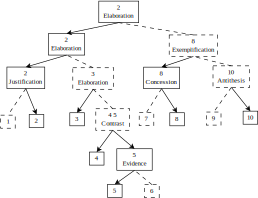
\includegraphics[width=.5\textwidth]{figures/approaches/rhet-tree.pdf} % % %[width=140mm]
		\caption{An example of a rhetorical tree \citep{98-marcu}.}
		\label{fig:rhet-tree}
	\end{center}
\end{figure}
The author uses seven metrics based on the rhetorical tree to find the best discourse interpretation similar to those of summaries: The clustering-based metric, the marker-based metric, the rhetorical-clustering-based metric, the shape-based metric, the title-based metric, the position-based metric and the connectedness-based metric.


\citet{14-kikuchi-al} propose a single document \ac{ats} based on nested tree structure. 
The authors exploit words dependency and rhetorical dependency  by constructing a nested tree composed of a document tree and a sentence tree. 
The document tree has sentences as nodes and head modifier relationships between sentences obtained by \ac{rst} as edges. 
The sentence tree has words as nodes connected by head modifier relationships between them obtained by the dependency parser.
The summarization is formulated as combinatorial optimization problem in order to trim the nested tree.

A more recent work using \ac{rst} is the work of \citet{16-goyal-eisenstein}, to fix the problems of local inference techniques which do not capture document-level structural regularities, and annotated training data.
So, the authors investigated the use SampleRank \citep{11-wick-al} structure learning algorithm as a potential solution to both problems.

\section{Machine learning (ML) approach}

Usually, machine learning approach is coupled with other approaches to improve and estimate their generation rules instead of fixing them manually.
It can solve the problem of combining features in statistical approach.
Many works have been conducted to generate summaries using machine learning, some focus on the choice of appropriate classification methods \citep{95-kupiec-al,02-osborne,05-yeh-al}, some try to solve the problems related to training phase, such as the absence of labeled corpora \citep{02-amini-gallinari}, others use heterogeneous features in their algorithms and try to combine them using machine learning \citep{08-wong-al,10-yatsko-al}. 

\subsection{As a tuning function}

\ac{ml} can be used with other approaches to tune certain parameters. 
It is mostly accompanied with statistical approach to solve the problem of estimating features weights, where these features scores are combined linearly into one score.
\citet{05-yeh-al} propose a method using genetic algorithm to estimate the features weights (sentence position, keywords, centroid and title similarity). 
Training a system on a corpus makes it dependent to the corpus's genre. 
A solution is to tune the features according to the input document's genre as suggested in \citep{10-yatsko-al}. 
45 features are used to train the system on three genres: scientific, newspaper, and artistic texts. 
The system can detect the genre of the input document and execute the adequate model of scoring. 

\subsection{As a decision function}

Given a corpus of documents with their extractive summaries, a machine learning algorithm can be used to decide if a unit (sentence mostly) belongs to the summary or not.
\citet{95-kupiec-al} propose an ATS system based on Bayes classification, in order to calculate the probability that a summary may contain a given sentence.
So, for each sentence $ s_i $, the probability that it belongs to a summary $ S $ using a features vector $ \overrightarrow{f} $ is given in Equation \ref{eq:bayes-kupiec}.
\begin{equation}
	\label{eq:bayes-kupiec}
	P(s_i \in S | \overrightarrow{f}) = %
	\frac{\prod\limits_{j = 1}^{|\overrightarrow{f}|} P(f_j | s_i \in S) * P(s_i \in S)}
	{\prod\limits_{j = 1}^{|\overrightarrow{f}|} P(f_j)}
\end{equation}
Where: 
$ P(s_i \in S) $ is a constant (so it can be emitted, since the probability is used for reordering), $ P(f_j | s_i \in S) $ and $ P(f_j) $ can be estimated from a corpus.
%
Choosing the right classification algorithm is another issue; for instance Bayes classification supposes features independence, which is not always the case.

From this point of view, \citet{02-osborne} uses a maximum entropy based classifier which, unfortunately, performs lower than Bayes' because it tends to reject a lot of sentences; but when he adds a prior probability, the method performs well and surpasses Bayes-based method.
His method, though, is not used to reorder sentences using the probability, but to classify them into two classes: summary sentences and other sentences.

\subsection{Bayesian topic models}

Topic models are based on identifying the main concepts from the input document(s) and find the relationship between them to construct a hierarchy. 
Words of each input document are assigned to a given number of topics, where a document is a mixture of different topics and each topic is a distribution of words. 
Bayesian topic models are quite sophisticated for multi-document summarization since they make difference between documents in contrast to most ATS methods which consider them as one giant document \citep{11-nenkova-mckeown}.
One of Bayesian topic models' advantages is their simplicity to incorporate different features, such as cue phrases used in \citep{08-eisenstein-barzilay} for unsupervised topic segmentation.


\citet{06-daumeiii-marcu} propose a query-driven muli-document summarization method using Bayesian topic models which is reported in \citep{11-nenkova-mckeown} as one of the first works in this direction.
In their method, the authors train their system to have three probability distributions: general English learning model ($ P^G $), background document language model ($ P^D $) for each one of the $ K $ available documents with $ S $ number of sentences and $ N $ number of words $ w $ in a sentence, and query language model ($ P^Q $) for each query $ q $ over a set of $ J $ queries.
Using this trained model, they estimate $ \pi $ using Expectation propagation \citep{01-minka}.
Figure~\ref{fig:btm-daumeiii} represents the graphical model of their method, where $ r $ is the relevance judgment,  $ z $ is the word-level indicator variables, $ \pi $ is the sentence level degrees, and $ \alpha $ is a Dirichlet distribution as prior over $ \pi $.
\begin{figure}[ht]
	\begin{center}
		\includegraphics{figures/approaches/btm-daumeiii.pdf} % % %[width=140mm]
		\caption{Bayesian Query-Focused Summarization Model proposed in \citep{06-daumeiii-marcu}.}
		\label{fig:btm-daumeiii}
	\end{center}
\end{figure}


\citet{11-celikyilmaz-hakkani} introduces \ac{ttm} which models topics as two levels: low-level topics which are distributions over words, and top-level topics which are correlations between these lower level topics given sentences.
One problem with \ac{ttm} is its incapability to differentiate general words from specific ones given a query. 
A Sentence containing general words, which are more frequent in document clusters, must have more chance to be included into the summary. 
The authors present an enriched \ac{ttm} (ETTM) generative process to sample words from high-level topics leading to three words distributions: low-level topics over corpus specific words, high-level topics over corpus general words, and background word distributions.

\citet{15-yang-al} argue that using expert summaries to indicate only two levels of topics limits the practical applications of \citet{11-celikyilmaz-hakkani}'s model, because we can draw many latent topics from multiple documents.
The availability of reference summaries and their quality as golden standards are two other challenges to this method. 
Furthermore, TTM does not take word dependency in consideration. 
To address these limits, they propose a new method called \ac{ctm} which is based on Bayesian topic model \ac{ttm}, hLDA model \citep{10-blei-al}, topical N-grams \citep{07-wang-al}, with some concepts of graph models. 

\subsection{Reinforcement learning (RL)}

%define reinforcement learning
Before presenting some \ac{ats} works based on \ac{rl}, lets first introduce \ac{rl} briefly. 
Given an agent in an environment, the former interacts with the latter via perception and action \citep{96-kaelbling-al}.
At each interaction, the agent perceives the current state $ s $ of its environment, among the set of possible states $ \mathcal{S} $.
Based on $ s $, the agent choose an action $ a $ from the set of actions it can perform on that state $ \mathcal{A}(s) $.
Of course, applying an action will change the environment's state to a new one $ s' $ resulting in a reward $ r $.
The agent's job is to learn an optimal policy $ \pi^* $, mapping states to actions $ p(a/s) $, that maximizes some long-run rewards.


\citet{12-ryang-abekawa} consider \ac{ats} extractive approach as a search problem. 
To our knowledge, They are the first to model the problem of constructing a summary as a \ac{rl} problem.
The state $ s = (S, A, f) $ is represented as a tuple of the current summary $ S $, a history of applied actions $ A $ and an indicator $ f \in \{0, 1 \} $ showing if it is terminal or not.
Thus, the initial state is represented as $ s_0 = (\emptyset,\emptyset, 0) $.
The authors define a function $ s: \phi(s) \in \mathbb{R}^d $ on the state, which is based only on the summary's feature $ \phi'(S) $ as given in Equation~\ref{eq:ryang-features}.
\begin{equation}
\label{eq:ryang-features}
\phi(s) = \left\lbrace 
\begin{array}{ll}
(\phi'(S), 0)^T & L(S) \le K \\
(0, 1)^T & otherwise \\
\end{array}
\right. 
\end{equation}
Where, $ K $ is the maximum size of a summary, $ L(S) $ is the current size of the summary and $ (0, 1)^T $ indicates that the summary violates the size constraint. 
In their experiments, the authors represent $ \phi'(S) $ as a vector of the following features: Coverage of important words, Coverage ratio, Redundancy ratio, Length ratio and Position. 
There are two types of actions: insert a unit (sentence) $ x_i $ referred to as $ insert_i $ and finish referred as $ finish $. 
%So, given an instant $ t $, the two types of transactions from a state $ s_t $ to another $ s_{t+1} $ using an action $ a_t $ are given in Equation~\ref{eq:ryang-actions}
%\begin{equation}
%\label{eq:ryang-actions}
%\begin{matrix}
%s_t & a_t  & s_{t+1} \\ 
%&\\
%
%\begin{pmatrix}
%S_t\\ 
%A_t\\ 
%0
%\end{pmatrix} & 
%\overset{insert_i}{\rightarrow} & 
%\begin{pmatrix}
%S_t \cup \{x_i\}\\ 
%A_t \cup \{ insert_i\}\\ 
%0
%\end{pmatrix} \\
%
%&\\
%
%\begin{pmatrix}
%S_t\\ 
%A_t\\ 
%0
%\end{pmatrix} & 
%\overset{finish}{\rightarrow} & 
%\begin{pmatrix}
%S_t \\ 
%A_t \cup \{ finish\}\\ 
%1
%\end{pmatrix} 
%\end{matrix}
%\end{equation}
The agent is rewarded only when it is in finish state; It is rewarded by the summary score $ score(S_t) $ if it does not violate the size limit, and it is penalized by a given value $ R_{penalty} $ otherwise.
The reward is represented in Equation~\ref{eq:ryang-reward}.
\begin{equation}
\label{eq:ryang-reward}
r_{t+1} = \left\lbrace 
\begin{array}{ll}
score(S_t) & a_t = finish \text{ and } L(S_t) \le K \\
- R_{penalty} & a_t = finish \text{ and } L(S_t) > K \\
0 & otherwise \\
\end{array}
\right. 
\end{equation}
The score of a summary $ S $ is a trade-off between its relevance $ Rel $ and redundancy $ Red $ as shown in Equation~\ref{eq:ryang-score}. 
\begin{equation}
\label{eq:ryang-score}
Score(S) = \sum\limits_{x_i \in S} \lambda_s Rel(x_i) - \sum\limits_{x_i, x_j \in S, i < j} (1 - \lambda_s) Red(x_i, x_j)
\end{equation}
Where $ Rel(x_i) $ is the cosine similarity between $ x_i $ and the document $ D $ plus a position-based score, $ Red(x_i, x_j) $ is the cosine similarity between these two units, and $ \lambda_s $ is a trad-off parameter set to $ 0.9 $. 
The policy is represented as a conditional distribution $ p(a|s;\theta,\tau) $ based on Boltzmann selection, which is parameterized by $ \theta $ and a temperature parameter $ \tau $.
The probability is calculated using $ r $ and $ \phi(s) $.
The authors use $ TD(\lambda) $ algorithm which is based on \ac{td} learning to estimate $ \theta $.


\citet{15-rioux-al} base their work on the method of \citet{12-ryang-abekawa}. 
They use an improved version of \ac{td} called \ac{sarsa} which, in addition to modeling state space, it models actions space too. 
Their reward function is immediate at every action to help the learner get immediate feedback.
It is similar to that of \citet{12-ryang-abekawa}, but the similarity function uses bi-grams instead of \ac{tfidf} and it incorporates ROUGE score.
%
Likewise, \citet{15-henss-al} follow the same method but with some changes. 
They use a different reward function based on reference summaries $ H_D $ and a set of features including ROUGE score during training.
Given a summary $ S_t $, the reward after performing and action leading to a summary $ S_{t+1} $ can be expressed as in Equation~\ref{eq:henss-reward}.
\begin{equation}
\label{eq:henss-reward}
r_{t} = Score(S_{t+1}; H_D) - Score(S_{t}; H_D)
\end{equation}
Where $ Score $ is a linear combination of the features scores.
Instead of using \ac{td} learning, the authors use Q-Learning to determine the value of the partial summary and the value of adding a new sentence to a summary state.
%Their method learns one global policy for a specific summarization task instead of one policy for each document cluster.

\ac{rl} can, also, be combined with deep learning to generate extractive summaries \citep{18-wu-hu}. 
The authors define a deep neural network model which takes as input the document $ d = (s_1, s_2, ..., s_n) $ composed on $ n $ sentences.
The model outputs a victor of binary decisions $ Y = (y_1, y_2, ..., y_n) $ indicating whether a sentence $ s_i $ belongs to the summary or not.
After training this model with supervised learning, it is trained again using \ac{rl} in order to incorporate coherence.


\subsection{Deep learning (DL)}

\ac{dl} has gained a lot of attention recently, even among \ac{ats} community.
It is based on large \ac{nn} which, eventually, needs a huge amount of data to be trained. 
It has been used for both extractive and abstractive \ac{ats}. 
We will start by presenting some extractive methods, then some abstractive ones.
%extractive

In \citep{12-liu-al,15-zhong-al}, the authors propose a query-oriented multi-document \ac{ats} method based on a \ac{dl} model.
The model contains three parts: concepts extraction, reconstruction validation and summary generation.
Concepts extraction is an encoder with 4 \ac{nn} layers which is fed with a vector of \ac{tf} representing a vocabulary with length $ V $ based on words appearing in the document topic set $ D $. 
Reconstruction validation is a decoder with 3 \ac{nn} layers which aims to reconstruct the input vectors. 
The last layer of Concepts extraction part is used with dynamic programming to seek most informative sentences. 

\citet{14-denil-al} use a hierarchical ConvNet architecture (CNN) divided into a sentence level and a document level.
The sentence level learns to represent sentences using their words and the document level learns to represent the input document using the first level. 
Then, these representations are used to score how pertinent a sentence can be towards the entire document.
Figure~\ref{fig:14-denil-al} represents the architecture used to infer document embedding from word embedding. 
First, word embeddings are concatenated into a sentence matrix which is transformed into a single vector using some operations. 
Then, the sentence embeddings are concatenated and transformed into a vector representing the document.
%
\begin{figure}[!ht]
	\begin{center}
		\includegraphics[width=.7\textwidth]{figures/approaches/14-denil-al.pdf} % % %[width=140mm]
		\caption{Inferring document embedding from word embedding in \citep{14-denil-al}.}
		\label{fig:14-denil-al}
	\end{center}
\end{figure}

In \citep{15-cao-al}, a \ac{r2n2} is used to rank sentences for multi-document summarization. 
The authors use two types of hand-crafted features as inputs: word features and sentence features. 
This enables the system to learn how to score sentences based on a hierarchical regression process which uses a parsing tree to score sentence constituents such as phrases. 

Like \citet{15-zhong-al}, \citet{17-yousefiAzar-hamey} propose an extractive query-oriented summarization method based on deep learning but for single-document \ac{ats}.
The main difference is the use of an unsupervised approach with deep \ac{ae} which was used in \citet{15-zhong-al} as a word filter rather than a sentence ranker. 
The AE, in this case, can learn different features rather than manually engineering them.
Furthermore, the authors investigate the effect of adding random noise to the local word representation vector on the summary.

In \citep{17-ren-al}, a neural network of two levels using contextual relations among sentences is proposed to improve sentence regression's performance. 
The first level captures sentence representations using a word-level attentive pooling convolutional neural network. 
Then, the second one constructs context representations using sentence-level attentive pooling recurrent neural network. 
These learning representations and the similarity of a sentence with its context are used to extract useful contextual features. 
The authors train the system to learn how to score a sentence to fit the ground truth of ROUGE-2.

%abstractive
To our knowledge, \citet{15-rush-al} are the first to successfully apply deep learning to abstractive \ac{ats}. 
Their system called NAMAS\footnote{NAMAS code: \url{https://github.com/facebookarchive/NAMAS} [October 03, 2017]} performs well on ``DUC-2004 shared task" corpus despite being tested using ROUGE metric which, mostly, encourages extractive summaries. 
The method uses a local attention-based model to generate each word of the summary $ y $ conditioned on the input sentence $ x $.
To do that, the model is trained to estimate a probability $ p(y_{i+1}|y_c, x; \theta) $ of generating a word $ y_{i+1} $ from a fixed vocabulary $ \mathcal{V} $ constructed from the input text. 
The probability is conditioned by the input sentence $ x $, a sequence of $ C $ words representing the last generated words, and parameters $ \theta $ representing word embedding matrix and weight matrices.
This method shows some limitations when it comes to input document and summary's size. 
It processes only documents with a size of about 500 words and produces a very short summary (about 75 characters). 

The previous work only generates summaries using input document's vocabulary without introducing out-of-vocabulary words.
To tackle this limitation, \citet{16-nallapati-al} also use an attention model in their encoder-decoder.
When they decode, they use only words that appear in the source document following a method called ``Large Vocabulary Trick" (LVT) \citep{15-jean-al}. 
Then, to introduce new words, they add a layer of ``word2vec nearest neighbor" in the input. 
The decision whether to use a word from the input or a new word based on the context is guaranteed by another layer they call ``Switching Generator/Pointer" layer \citep{15-luong-al,15-vinyals-al}.


\citet{17-ling-rush} try to fix the problem of speed when long source sequences (document summarization) are processed using sequence-to-sequence models with attention.
So, they use a two layer hierarchical attention; Where the first layer's function is to select one or more important chunks from the input document using hard attention, then feed it/them into the second layer using sequence-to-sequence model.
They use reinforcement learning to train the hard attention model.
The method shows promise to scale up existing methods into larger inputs, but fails to beat the standard sequence-to-sequence model. 



%\section{Sentence compression}
%
%
%The compression or reduction of sentences is the elimination of non informative parts, especially when the sentence is too long.
%\citet{99-jing-mckeown} confirm that the compression is often used by professional summarizers. 
%In fact, they found out that 78\% of summaries sentences are borrowed from the original document, and that half of them have been compressed.
%
%In \citep{02-knight-marcu}, two statistical compression methods are proposed: using the noisy channel model, and using decision trees.
%The first method supposes that the input sentence was short but has been bloated with additional words. 
%For a given long sentence, a syntactic tree is produced to which a quality score is attributed.
%It is calculated using \ac{pcfg} scores and the probabilities of next sentence calculated with bi-gram language model. 
%They measure the likelihood of transforming a wide tree to a reduced one using statistics gathered from a corpus of documents and their summaries.
%The second method is based on decision trees used to learn the different rules to reduce sentences.
%
%Likewise, in their statistical compression method, \citet{07-Zajic-al} consider a sentence to be a headline distorted by adding other words to it. 
%They use \ac{hmm} to represent the problem and finding the headline which maximizes the likelihood of this headline generating the sentence. 
%This likelihood is estimated using probabilities that a word is followed by another in a corpus of English headlines taken from TIPSTER corpus. 
%The authors propose another rule-based method where they use a parser to get the syntactic representation of the sentence, used to remove some components such as temporal expressions, modal verbs, complimentizer \textit{that}, etc.
%The compression is executed iteratively by removing one component at a time, outputting the compressed sentence into the extraction module.
%
%Other methods have been proposed to improve sentences compression using not only one sentence but using similar sentences.
%In \citep{08-cohn-lapata}, instead of shortening the sentence by removing words or components, the authors introduce additional steps as substitution, reordering, and insertion.
%In \citep{10-filippova}, a method is proposed to summarize a group of related sentences to a reduced one.
%In this method, the sentences are represented by one graph which is used to generate a reduced summary by following the shortest path.
%
%Deep learning has been applied in order to compress sentences. 
%\citet{15-filippova-al} use \ac{lstm} in order to perform a deletion-based sentence compression. 
%The method performs very well either in term of readability or informativeness even without affording syntactic information (PoS, NE tags and dependencies).
%%
%The same method is used in \citep{17-hasegawa-al} to compress Japanese sentences, but with some changes. 
%These modifications are based on three Japanese language characteristics: 
%\begin{itemize}
%	\item frequent verbs are nominalized and nouns are abbreviated;
%	\item a non verb can be a root node
%	\item easily estimated subjects and objects are omitted
%\end{itemize}


\section{Discussion}

We based our taxonomy on resources dependency: is a method based on some corpora? does it depend on some language toolkits? how much calculation power it needs?
Our intention is to classify \ac{ats} methods based on resource availability and the effort they take to be implemented. 
In this section, we will try to discuss the capacity of each approach to support multilingualism.

Statistical features based methods were the first introduced in ATS. 
Features like term frequency, position and length are language independent and are good indicators of sentence relevance. 
A statistical approach does not need much language dependent tools; just some basic \ac{nlp} tasks such as sentence segmentation, tokenizaion, stop word elimination, and stemming. 
Mostly, it is easy to be implemented and does not need a lot of processing power.
The statistical features are combined together in hope to better capture a sentence's relevance. 
This leads to a more complicated problem which is how to combine them, and how much amount of influence of each one. 
The problem can be solved by combining them linearly, and set their weights through experiments using a corpus or estimate them using machine learning.
Either way, we will have another problem which is language dependency. 

Graph-based approach seeks to exploit the shared information between sentences. 
It is a bottom-up method which discusses the similarity problem from the perspective of content structure \citep{15-yang-al}. 
It can be language-independent using just lexical similarities (mostly, cosine similarity) and statistical features. 
But, some room for improvement can be done by considering more language dependent similarities such as semantic similarity. 
Also, the model can be improved using machine learning, by introducing prior probabilities into the equation, as in \citep{08-liu-al}.
Processing a great amount of text using iterative graphs can consume more processing power; this should be investigated to better understand how far this approach can go.

Linguistic approach is more powerful than the statistic one in term of expressiveness, because it integrates richer features of the input text. 
Also, it can be used either for extractive or abstractive summarization.  
The problem with this approach is the lack of appropriate NLP tools for certain languages. 
It can be as simple as using sentence components (verbs, nouns, etc.) as statistical features, or as hard as using sentence structure and its relationships with others to generate a new text. 
Mostly, it is harder to be implemented and takes more time to generate a summary. 
\citet{11-nenkova-mckeown} suggests using linguistic methods as a post-processing task to improve linguistic quality of the generated summary rather than a processing one.
According to the authors, it is unclear how much this approach can improve content selection compared to the methods using no linguistic relations. 

All approaches discussed previously can be ameliorated using machine learning (ML).
On the other hand, they can loose multilingual property unless the system is trained on as many languages as possible. 
Still the problem of corpus domain; training your system on news articles does not mean it can handle fiction as good as it does with news.
Also, collecting labeled corpora for one language can be a very hard work, let alone many languages. 
Some works seek to use unlabeled data, and some propose auto-supervised methods such as \citep{02-amini-gallinari}.

%Sentence compression seeks to get rid of non informative parts allowing us to have shorter sentences. 
%It can be used as a post-processing task after generating a summary, which will eliminate more redundancy and allows more space for other sentences to be included. 
%It is a language dependent task which cannot be used alone to have a summary, but in conjunction of other approaches.

We tried to summarize all the above discussion in Table~\ref{tab:app-comp}.
The table shows some advantages and disadvantages of each approach, some encountered problems and their eventual fixes.
\begin{table}[ht]
	\caption{Comparison between different ATS approaches.\label{tab:app-comp}}
	\begin{tabular}{p{.12\textwidth}p{.25\textwidth}p{.25\textwidth}p{.25\textwidth}}
		\hline\hline\noalign{\smallskip}
		
		Approach & pros (+) \& cons (-) & problems & fixes \\
		\noalign{\smallskip}\hline\noalign{\smallskip}
		
		%==============STATISTICAL================
		Statistical 
		& 
		+ less resources \newline 
		+ simple \& fast \newline
		- readability
		& 
		* features combination \newline
		* relevancy \newline 
		* redundancy in sentences
		& 
		* machine learning \newline
		* linguistic features \newline 
		* compression
		\\
		
		\hline\noalign{\smallskip}
		
		%==============GRAPH================
		Graph 
		& 
		+ less resources \newline 
		+ simple \newline
		+ coherence \newline
		- processing power
		& 
		* sentences similarity \newline 
		* sentences \& documents properties
		& 
		* tf-idf, semantic \newline 
		* statistical \& linguistic features, sentence-document similarity, temporal property
		\\
		
		\hline\noalign{\smallskip}
		
		%==============LINGUISTIC================
		Linguistic 
		& 
		+ more accurate  \newline 
		+ abstractive ATS  \newline 
		- resources (toolkits) \newline 
		- complex \newline
		- processing power
		& 
		* generation rules
		&
		* machine learning 
		\\
		
		\hline\noalign{\smallskip}
		
		%==============MT================
		Machine learning 
		& 
		+ deducing rules automatically \newline
		- lack of corpora \newline
		& 
		* labeled corpora \newline
		* corpora insufficiency
		& 
		* reinforcement learning \newline
		* corpora creation
		\\
		
		\hline\noalign{\smallskip}
		
%		%==============Compression================
%		Compression 
%		& 
%		+ less redundancy \newline
%		- sentence level
%		& 
%		* sentence level
%		& 
%		* fuse with other approaches as a post-processing task
%		\\
%		
%		\noalign{\smallskip}\hline\hline
	\end{tabular} 
\end{table}
